% Author: PokMan Ho
% Script: apdx.tex
% Desc: MRes thesis appendix section
% Input: none
% Output: none
% Arguments: 0
% Date: Jan 2020

\documentclass[../thesis.tex]{subfiles} %% use packages & commands as this main file

\begin{document}
\section{Appendix}
\beginSupp
%this is an appendix

\subsection{features comparison between models}
\begin{table}[H]
\begin{tiny}
    \centering
    \caption[Model features comparison]{Table of features comparison (18 features) between model in this project with aquatic slab models (23 models) and two terrestrial nutrient cycle models}
    \csvautotabular[]{media/modComp1.csv}\\
    \vspace{.5cm}
    \csvautotabular[]{media/modComp2.csv}\\
    \vspace{.5cm}
    \csvautotabular[]{media/modComp3.csv}
    \label{modComp}
\end{tiny}
\end{table}

\subsection{temperature-standardization}
The procedure included two parts.  Parameter values collected from literature were temperature-tagged.  For parameters with very limited data points, majority of the data were collected under 23-25$^o$C.  Hence this study chose 23$^o$C as the standard reference to investigate with the proposed model.

Growth rate data was obtained from ``BioTrait" database\autocite{della2013thermal}.  Six filters were applied to extract published aquatic microbial P or B species entries which were identified to species level.  The matched data set was further filtered to eliminate entries reported no growth because these records could not reflect the temperature effect using the Arrhenius Equation.

\begin{equation}
    A = A_0e^{-\dfrac{E_a}{k(T_C+273.15)}}
    \label{arrEq}
\end{equation}

which $A$ is rate standardised in data and $A_0$ is the standardisation constant with the same unit, $E_a$ is the activation energy with unit eV, $k$ is Boltzmann constant from Scipy (v1.4.1) package under unit eV/K and $T_C$ is the temperature of the organism measured from the data with unit ($^oC$).

Activation energies for phytoplanktons and bacterial decomposers are 0.32eV and 0.66eV respectively.\autocite{regaudie2012temperature}  Standardised rate unit in data was initially ``$sec^{-1}$" and the unit was re-standardised to ``$day^{-1}$" for this study (Fig.\ref{growStdVal}).

\begin{figure}[H]
    \centering
    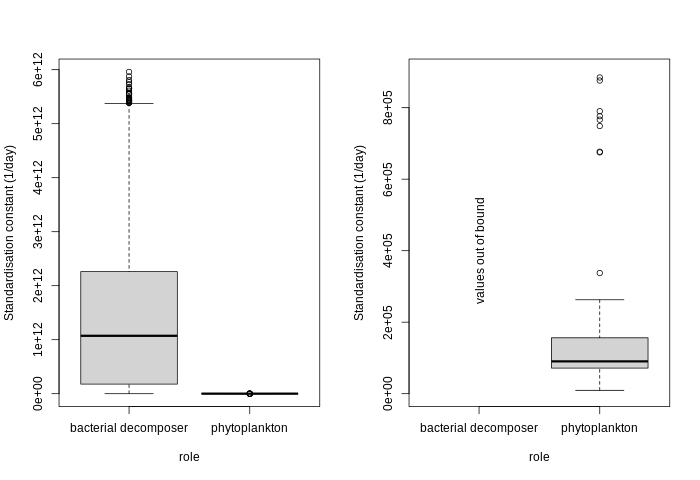
\includegraphics[width=\linewidth]{../result/stdCst.png}
    \caption[Boxplot of standardised $A_0$]{Boxplots of $A_0$ for P and B with unit ``$day^{-1}$"}
    \label{growStdVal}
\end{figure}

The interquartile ranges in Fig.\ref{growStdVal} for the two organism types were used to standardise the growth rates data of respective categories.

\subsection{phytoplankton growth rates}


\subsection{bacterial decomposer clearance rates}
For growth rate data, values were standardised

These are terms $\gP$ and $\gB$ respectively.  Values calculated from this section also used to calculate $\ePR$.  Thermal performance data was obtained from ``BioTrait" database\autocite{della2013thermal} with 25826 entries and 155 columns of data and descriptions (original, standardised values and units with citations).  Six filters were applied to the data, extracting data entries that were published and about aquatic species growth rates that were identified to species level and being either microbial phytoplankton or bacterial decomposer.  The resultant data was around 3.2K rows.  The intermediate data was further filtered to remove any standardised growth rate record with no growth because the purpose of this section is to get standardization constants based on temperature.  Since data with no growth would eliminate temperature factor during standardisation process, they are eliminated with logical reason.  The final growth rate data was standardised to specific growth rate based on seconds (sec$^{-1}$) with different empirical temperatures given by the respective experiments.

Standardisation was using Arrhenius Equation

\subsection{non-respired carbon fraction for phytoplankton}
This is the term $\ePR$ which was calculated using the summary of linear equations from \autocite{j1989respiration} and result of $\gP$ calculations.  Intercepts, slope values and their respective experimental temperatures were collected from respiration-growth analysis of the above paper.  Only entries from experiments with temperature ranging 23-25$^oC$ are extracted because it is the temperature range for all other parameters in this model (Table \ref{varInTab}).

Growth rates for phytoplanktons at 23$^oC$ were calculated from Eqn.\ref{arrEq}.  The non-respired fraction of carbon ($n(R')$) was calculated as

\begin{equation}
    P(R') = 1-P(R) = 1-\dfrac{\Bar{\text{intercept}}+\Bar{\text{slope}}\cdot\Bar{\gP}}{\Bar{\gP}}
    \label{ePReqn}
\end{equation}

\subsection{non-respired carbon fraction for bacterial decomposer}
This is the term $\eBR$ calculated from Fig.1b and glucose recovery rate values of \autocite{cochran1988estimation}.  This paper is also the only publication with values associated with its respected parameter in the model.  In the figure a net 100mg of carbon originated from straw material was recovered per gram of straw at around 24-28 days (from day 0).  At that period, the recovery rate of carbon released by respiration originated from external glucose was 80\%.  Since in the environment carbon source was either external glucose or straw, the respired carbon fraction is $\dfrac{100\cdot10^{-3}}{28\cdot(1-0.8)}$ and the non-respired carbon fraction is (1-[respired fraction]).

\subsection{maximum limit for intraspecific interference of phytoplankton}
This is the term $\aP$, which the maximum value of the wild scan was capped at 0.4.\autocite{de2007biofixation}  It is because logically higher temperature would lead to higher growth rate and hence a more intense competition.  So a higher death related to the intraspecific interference is associated.  Since the value measured in the paper was at 30$^oC$, the relative intraspecific interference value should logically be under this value.  Adding to the fact that the above paper is the only paper published with a value of intraspecific interference, it is unjustified to assume an Arrhenius equation can be applied to guesstimate the respective value at the model's temperature range setting with one data entry.

\end{document}
